
%% bare_conf.tex
%% V1.3
%% 2007/01/11
%% by Michael Shell
%% See:
%% http://www.michaelshell.org/
%% for current contact information.
%%
%% This is a skeleton file demonstrating the use of IEEEtran.cls
%% (requires IEEEtran.cls version 1.7 or later) with an IEEE conference paper.
%%
%% Support sites:
%% http://www.michaelshell.org/tex/ieeetran/
%% http://www.ctan.org/tex-archive/macros/latex/contrib/IEEEtran/
%% and
%% http://www.ieee.org/

%%*************************************************************************
%% Legal Notice:
%% This code is offered as-is without any warranty either expressed or
%% implied; without even the implied warranty of MERCHANTABILITY or
%% FITNESS FOR A PARTICULAR PURPOSE! 
%% User assumes all risk.
%% In no event shall IEEE or any contributor to this code be liable for
%% any damages or losses, including, but not limited to, incidental,
%% consequential, or any other damages, resulting from the use or misuse
%% of any information contained here.
%%
%% All comments are the opinions of their respective authors and are not
%% necessarily endorsed by the IEEE.
%%
%% This work is distributed under the LaTeX Project Public License (LPPL)
%% ( http://www.latex-project.org/ ) version 1.3, and may be freely used,
%% distributed and modified. A copy of the LPPL, version 1.3, is included
%% in the base LaTeX documentation of all distributions of LaTeX released
%% 2003/12/01 or later.
%% Retain all contribution notices and credits.
%% ** Modified files should be clearly indicated as such, including  **
%% ** renaming them and changing author support contact information. **
%%
%% File list of work: IEEEtran.cls, IEEEtran_HOWTO.pdf, bare_adv.tex,
%%                    bare_conf.tex, bare_jrnl.tex, bare_jrnl_compsoc.tex
%%*************************************************************************

% *** Authors should verify (and, if needed, correct) their LaTeX system  ***
% *** with the testflow diagnostic prior to trusting their LaTeX platform ***
% *** with production work. IEEE's font choices can trigger bugs that do  ***
% *** not appear when using other class files.                            ***
% The testflow support page is at:
% http://www.michaelshell.org/tex/testflow/



% Note that the a4paper option is mainly intended so that authors in
% countries using A4 can easily print to A4 and see how their papers will
% look in print - the typesetting of the document will not typically be
% affected with changes in paper size (but the bottom and side margins will).
% Use the testflow package mentioned above to verify correct handling of
% both paper sizes by the user's LaTeX system.
%
% Also note that the "draftcls" or "draftclsnofoot", not "draft", option
% should be used if it is desired that the figures are to be displayed in
% draft mode.
%
\documentclass[conference]{IEEEtran}

% Add the compsoc option for Computer Society conferences.
%
% If IEEEtran.cls has not been installed into the LaTeX system files,
% manually specify the path to it like:
% \documentclass[conference]{../sty/IEEEtran}





% Some very useful LaTeX packages include:
% (uncomment the ones you want to load)


% *** MISC UTILITY PACKAGES ***
%
%\usepackage{ifpdf}
% Heiko Oberdiek's ifpdf.sty is very useful if you need conditional
% compilation based on whether the output is pdf or dvi.
% usage:
% \ifpdf
%   % pdf code
% \else
%   % dvi code
% \fi
% The latest version of ifpdf.sty can be obtained from:
% http://www.ctan.org/tex-archive/macros/latex/contrib/oberdiek/
% Also, note that IEEEtran.cls V1.7 and later provides a builtin
% \ifCLASSINFOpdf conditional that works the same way.
% When switching from latex to pdflatex and vice-versa, the compiler may
% have to be run twice to clear warning/error messages.






% *** CITATION PACKAGES ***
%
%\usepackage{cite}
% cite.sty was written by Donald Arseneau
% V1.6 and later of IEEEtran pre-defines the format of the cite.sty package
% \cite{} output to follow that of IEEE. Loading the cite package will
% result in citation numbers being automatically sorted and properly
% "compressed/ranged". e.g., [1], [9], [2], [7], [5], [6] without using
% cite.sty will become [1], [2], [5]--[7], [9] using cite.sty. cite.sty's
% \cite will automatically add leading space, if needed. Use cite.sty's
% noadjust option (cite.sty V3.8 and later) if you want to turn this off.
% cite.sty is already installed on most LaTeX systems. Be sure and use
% version 4.0 (2003-05-27) and later if using hyperref.sty. cite.sty does
% not currently provide for hyperlinked citations.
% The latest version can be obtained at:
% http://www.ctan.org/tex-archive/macros/latex/contrib/cite/
% The documentation is contained in the cite.sty file itself.






% *** GRAPHICS RELATED PACKAGES ***
%
\ifCLASSINFOpdf
  \usepackage[pdftex]{graphicx}
  % declare the path(s) where your graphic files are
  % \graphicspath{{../pdf/}{../jpeg/}}
  % and their extensions so you won't have to specify these with
  % every instance of \includegraphics
  % \DeclareGraphicsExtensions{.pdf,.jpeg,.png}
\else
  % or other class option (dvipsone, dvipdf, if not using dvips). graphicx
  % will default to the driver specified in the system graphics.cfg if no
  % driver is specified.
  % \usepackage[dvips]{graphicx}
  % declare the path(s) where your graphic files are
  % \graphicspath{{../eps/}}
  % and their extensions so you won't have to specify these with
  % every instance of \includegraphics
  % \DeclareGraphicsExtensions{.eps}
\fi
% graphicx was written by David Carlisle and Sebastian Rahtz. It is
% required if you want graphics, photos, etc. graphicx.sty is already
% installed on most LaTeX systems. The latest version and documentation can
% be obtained at: 
% http://www.ctan.org/tex-archive/macros/latex/required/graphics/
% Another good source of documentation is "Using Imported Graphics in
% LaTeX2e" by Keith Reckdahl which can be found as epslatex.ps or
% epslatex.pdf at: http://www.ctan.org/tex-archive/info/
%
% latex, and pdflatex in dvi mode, support graphics in encapsulated
% postscript (.eps) format. pdflatex in pdf mode supports graphics
% in .pdf, .jpeg, .png and .mps (metapost) formats. Users should ensure
% that all non-photo figures use a vector format (.eps, .pdf, .mps) and
% not a bitmapped formats (.jpeg, .png). IEEE frowns on bitmapped formats
% which can result in "jaggedy"/blurry rendering of lines and letters as
% well as large increases in file sizes.
%
% You can find documentation about the pdfTeX application at:
% http://www.tug.org/applications/pdftex





% *** MATH PACKAGES ***
%
%\usepackage[cmex10]{amsmath}
% A popular package from the American Mathematical Society that provides
% many useful and powerful commands for dealing with mathematics. If using
% it, be sure to load this package with the cmex10 option to ensure that
% only type 1 fonts will utilized at all point sizes. Without this option,
% it is possible that some math symbols, particularly those within
% footnotes, will be rendered in bitmap form which will result in a
% document that can not be IEEE Xplore compliant!
%
% Also, note that the amsmath package sets \interdisplaylinepenalty to 10000
% thus preventing page breaks from occurring within multiline equations. Use:
%\interdisplaylinepenalty=2500
% after loading amsmath to restore such page breaks as IEEEtran.cls normally
% does. amsmath.sty is already installed on most LaTeX systems. The latest
% version and documentation can be obtained at:
% http://www.ctan.org/tex-archive/macros/latex/required/amslatex/math/





% *** SPECIALIZED LIST PACKAGES ***
%
%\usepackage{algorithmic}
% algorithmic.sty was written by Peter Williams and Rogerio Brito.
% This package provides an algorithmic environment fo describing algorithms.
% You can use the algorithmic environment in-text or within a figure
% environment to provide for a floating algorithm. Do NOT use the algorithm
% floating environment provided by algorithm.sty (by the same authors) or
% algorithm2e.sty (by Christophe Fiorio) as IEEE does not use dedicated
% algorithm float types and packages that provide these will not provide
% correct IEEE style captions. The latest version and documentation of
% algorithmic.sty can be obtained at:
% http://www.ctan.org/tex-archive/macros/latex/contrib/algorithms/
% There is also a support site at:
% http://algorithms.berlios.de/index.html
% Also of interest may be the (relatively newer and more customizable)
% algorithmicx.sty package by Szasz Janos:
% http://www.ctan.org/tex-archive/macros/latex/contrib/algorithmicx/




% *** ALIGNMENT PACKAGES ***
%
%\usepackage{array}
% Frank Mittelbach's and David Carlisle's array.sty patches and improves
% the standard LaTeX2e array and tabular environments to provide better
% appearance and additional user controls. As the default LaTeX2e table
% generation code is lacking to the point of almost being broken with
% respect to the quality of the end results, all users are strongly
% advised to use an enhanced (at the very least that provided by array.sty)
% set of table tools. array.sty is already installed on most systems. The
% latest version and documentation can be obtained at:
% http://www.ctan.org/tex-archive/macros/latex/required/tools/


%\usepackage{mdwmath}
%\usepackage{mdwtab}
% Also highly recommended is Mark Wooding's extremely powerful MDW tools,
% especially mdwmath.sty and mdwtab.sty which are used to format equations
% and tables, respectively. The MDWtools set is already installed on most
% LaTeX systems. The lastest version and documentation is available at:
% http://www.ctan.org/tex-archive/macros/latex/contrib/mdwtools/


% IEEEtran contains the IEEEeqnarray family of commands that can be used to
% generate multiline equations as well as matrices, tables, etc., of high
% quality.


%\usepackage{eqparbox}
% Also of notable interest is Scott Pakin's eqparbox package for creating
% (automatically sized) equal width boxes - aka "natural width parboxes".
% Available at:
% http://www.ctan.org/tex-archive/macros/latex/contrib/eqparbox/





% *** SUBFIGURE PACKAGES ***
% \usepackage[tight,footnotesize]{subfigure}
% subfigure.sty was written by Steven Douglas Cochran. This package makes it
% easy to put subfigures in your figures. e.g., "Figure 1a and 1b". For IEEE
% work, it is a good idea to load it with the tight package option to reduce
% the amount of white space around the subfigures. subfigure.sty is already
% installed on most LaTeX systems. The latest version and documentation can
% be obtained at:
% http://www.ctan.org/tex-archive/obsolete/macros/latex/contrib/subfigure/
% subfigure.sty has been superceeded by subfig.sty.



%\usepackage[caption=false]{caption}
%\usepackage[font=footnotesize]{subfig}
% subfig.sty, also written by Steven Douglas Cochran, is the modern
% replacement for subfigure.sty. However, subfig.sty requires and
% automatically loads Axel Sommerfeldt's caption.sty which will override
% IEEEtran.cls handling of captions and this will result in nonIEEE style
% figure/table captions. To prevent this problem, be sure and preload
% caption.sty with its "caption=false" package option. This is will preserve
% IEEEtran.cls handing of captions. Version 1.3 (2005/06/28) and later 
% (recommended due to many improvements over 1.2) of subfig.sty supports
% the caption=false option directly:
%\usepackage[caption=false,font=footnotesize]{subfig}
%
% The latest version and documentation can be obtained at:
% http://www.ctan.org/tex-archive/macros/latex/contrib/subfig/
% The latest version and documentation of caption.sty can be obtained at:
% http://www.ctan.org/tex-archive/macros/latex/contrib/caption/




% *** FLOAT PACKAGES ***
%
%\usepackage{fixltx2e}
% fixltx2e, the successor to the earlier fix2col.sty, was written by
% Frank Mittelbach and David Carlisle. This package corrects a few problems
% in the LaTeX2e kernel, the most notable of which is that in current
% LaTeX2e releases, the ordering of single and double column floats is not
% guaranteed to be preserved. Thus, an unpatched LaTeX2e can allow a
% single column figure to be placed prior to an earlier double column
% figure. The latest version and documentation can be found at:
% http://www.ctan.org/tex-archive/macros/latex/base/



%\usepackage{stfloats}
% stfloats.sty was written by Sigitas Tolusis. This package gives LaTeX2e
% the ability to do double column floats at the bottom of the page as well
% as the top. (e.g., "\begin{figure*}[!b]" is not normally possible in
% LaTeX2e). It also provides a command:
%\fnbelowfloat
% to enable the placement of footnotes below bottom floats (the standard
% LaTeX2e kernel puts them above bottom floats). This is an invasive package
% which rewrites many portions of the LaTeX2e float routines. It may not work
% with other packages that modify the LaTeX2e float routines. The latest
% version and documentation can be obtained at:
% http://www.ctan.org/tex-archive/macros/latex/contrib/sttools/
% Documentation is contained in the stfloats.sty comments as well as in the
% presfull.pdf file. Do not use the stfloats baselinefloat ability as IEEE
% does not allow \baselineskip to stretch. Authors submitting work to the
% IEEE should note that IEEE rarely uses double column equations and
% that authors should try to avoid such use. Do not be tempted to use the
% cuted.sty or midfloat.sty packages (also by Sigitas Tolusis) as IEEE does
% not format its papers in such ways.





% *** PDF, URL AND HYPERLINK PACKAGES ***
%
\usepackage{url}
% url.sty was written by Donald Arseneau. It provides better support for
% handling and breaking URLs. url.sty is already installed on most LaTeX
% systems. The latest version can be obtained at:
% http://www.ctan.org/tex-archive/macros/latex/contrib/misc/
% Read the url.sty source comments for usage information. Basically,
% \url{my_url_here}.





% *** Do not adjust lengths that control margins, column widths, etc. ***
% *** Do not use packages that alter fonts (such as pslatex).         ***
% There should be no need to do such things with IEEEtran.cls V1.6 and later.
% (Unless specifically asked to do so by the journal or conference you plan
% to submit to, of course. )


% correct bad hyphenation here
\hyphenation{op-tical net-works semi-conduc-tor agri-culture}

\begin{document}
%
% paper title
% can use linebreaks \\ within to get better formatting as desired
\title{Crop Yield Prediction using Supervised Statistical and Machine Learning Techniques}


% author names and affiliations
% use a multiple column layout for up to three different
% affiliations
\author{
\IEEEauthorblockN{Prajna Kandarpa}
\IEEEauthorblockA{ Mechanical and Mechatronics Engineering\\
University of Waterloo\\
Waterloo, Canada\\
Email: spspkand@uwaterloo.ca}
% \IEEEauthorblockN{Author 2}
% \IEEEauthorblockA{Systems Desing Engineering\\
% University of Waterloo\\
% Waterloo, Canada\\
% Email: author2@uwaterloo.ca}
}

% conference papers do not typically use \thanks and this command
% is locked out in conference mode. If really needed, such as for
% the acknowledgment of grants, issue a \IEEEoverridecommandlockouts
% after \documentclass

% for over three affiliations, or if they all won't fit within the width
% of the page, use this alternative format:
% 
%\author{\IEEEauthorblockN{Michael Shell\IEEEauthorrefmark{1},
%Homer Simpson\IEEEauthorrefmark{2},
%James Kirk\IEEEauthorrefmark{3}, 
%Montgomery Scott\IEEEauthorrefmark{3} and
%Eldon Tyrell\IEEEauthorrefmark{4}}
%\IEEEauthorblockA{\IEEEauthorrefmark{1}School of Electrical and Computer Engineering\\
%Georgia Institute of Technology,
%Atlanta, Georgia 30332--0250\\ Email: see http://www.michaelshell.org/contact.html}
%\IEEEauthorblockA{\IEEEauthorrefmark{2}Twentieth Century Fox, Springfield, USA\\
%Email: homer@thesimpsons.com}
%\IEEEauthorblockA{\IEEEauthorrefmark{3}Starfleet Academy, San Francisco, California 96678-2391\\
%Telephone: (800) 555--1212, Fax: (888) 555--1212}
%\IEEEauthorblockA{\IEEEauthorrefmark{4}Tyrell Inc., 123 Replicant Street, Los Angeles, California 90210--4321}}




% use for special paper notices
%\IEEEspecialpapernotice{(Invited Paper)}




% make the title area
\maketitle


\begin{abstract}
Neural Networks and Multiple Adaptive Regressive Splines (MARS), were used to predict crop yield for cereals for the country of India. Historical annual cereal yield data from 1960-2010 for the country of India was used as target data with seasonal mean temperatures, precipitation and arable land size as predictors. The two models were trained with this data and their predictions were compared with the actual yields as well as the performance of more complex crop models. 
\end{abstract}

\IEEEpeerreviewmaketitle



\section{Introduction}
Climate change has brought about increasingly chaotic weather patterns all over the planet making national economic and resource planning difficult for researchers, independent contractors and government organizations. These entities are therefore paying increased attention to the crop forecasts of major food-exporting countries as well as to their own domestic food production. Given the increased volatility of food markets and the rising incidence of climatic extremes affecting food production, food price spikes may increase in prevalence in future years \cite{iizumi2013prediction}. As such, complex models that can simulate ensemble effects from climate and soil conditions while accounting for geographical variability have assumed paramount importance. Crop growth models perform an abstraction of the dynamic mechanistic of the plant’s physiological stages by fitting them into a mathematical model \cite{Gonzalez-Sanchez2014}.

Recent research in this area has sought to build statistical models that perform just as well at forecasting yields as the complex models. Rauff (2015) \cite{Rauff2015} talk about how crop models can be used to understand the effects of climate change such as elevated nitrogen levels, CO2 levels, temperature and precipitation changes on crop development, growth and yield. For example, sudden onset of warm and humid conditions can lead to plant disease proliferation and cause crop yield loss and financial setbacks for farmers and geographical regions. It is a difficult task to produce a comprehensible, operational representation of a part of reality, which grasps the essential elements and mechanisms of that real world system and even more demanding, when the complex systems encountered in environmental management \cite{Rauff2015}.

A few kinds of crop models have been developed so far, ranging from empirical models to explanatory models. A widely used approach to this prediction problem is to rely on numerical models that emulate the main processes of crop growth and development. Lobell et al (2010)\cite{Lobell2010} state that these models are typically developed and tested using experimental trials and thus offer the distinct advantage of leveraging decades of research on crop physiology and reproduction, agronomy, and soil science, among other disciplines. Yet these models also require extensive input data on cultivar (plant varieties produced by selective breeding), management, and soil conditions that are unavailable in many parts of the world. 

The presence of all the data required for these models still requires calibration, which is difficult due to the high amount of uncertainty in the model parameters. Often, parameter uncertainty is ignored in such complex models and parameter values are picked through subjective deliberation. Iizumi et al. (2009) estimated distributions of parameter values from Markov Chain Monte Carlo techniques with the widths of the distributions reflecting the inability of historical rice, maize yield datasets to effectively constrain parameter values. They found that parameter uncertainties translated to larger uncertainties in projecting yield responses to climate change. They concluded that uncertainty of climate change impact assessment on crop yield may increase if future climate projections are fed to crop models with parameters optimized under current climate conditions \cite{Iizumi2009}.

Statistical models, on the other hand, trained with historical crop yield data, and made of relatively simple linear regression ensembles provide  a common alternative to the process based models described above. These methods include the following:
\begin{enumerate}
  \item time series methods - based on time series data from a single point or geographical area.
  \item panel methods - these methods rely on variations in both time and feature space. 
  \item cross sectional methods - based solely on variations in space.
\end{enumerate}
Time series methods are often limited by availability of data but have the advantage of capturing the variability for the chosen location. Panel and cross-sectional methods assume common parameter values across all locations and are prone to errors from omission of features like soil conditions or fertilizer uptake. The main advantages of statistical models are their limited reliance on field calibration data, and their transparent assessment of model uncertainties. For example, if a model does a poor job of representing crop yield responses to climate, this will be reflected in a low coefficient of determination ($R^2$) between modeled and observed quantities, as well as a large confidence interval around model coefficients and predictions. Although process-based models could in theory be accompanied with similar statistics, in practice they rarely are \cite{Lobell2010}. A few shortcomings with statistical models include co-linearity problems and assumptions of stationarity of the underlying ecological processes, which is an extremely important problem due to rapidly changing ecologies on the planet as a result of global warming. 

Lobell et al.\cite{Lobell2010} recognized the need for a systematic evaluation of statistical methods in predicting crop yields to climate and recommended that efforts be made to determine the specific conditions under which their predictions are likely to be misleading. This would help in quantifying the common errors that arise from using these simpler if imperfect approaches. Researchers \cite{Shi2013} \cite{lobell2009climate} have found that statistical models work best at large spatio-temporal scales like national or regional levels. Other researchers have highlighted the difference between understanding the impact of climate change on crop growth and on crop yields. Predicting crop yields involves understanding predictors that aren't reflected in the physiological crop growth models explaining their inability to reliably predict crop yields. This problem maybe considered as one of dimensionality reduction where multiple predictors need to be aggregated at regional, provincial and national levels and temporal scales like monthly or seasonal climatic variable changes.
\subsection{Objective}
The main goal of this report is to evaluate the accuracy of context unaware statistical models at accounting for the uncertainty found in the task of crop yield prediction. Statistical models that use Neural Networks and Multiple Adaptive Regressive Splines are to be built using historical annual crop yield, seasonal temperature and precipitation levels and assess their accuracy at predicting yields using measures such as error bounds, confidence intervals on predictions and compare these measures of variability with similar measures obtained by crop growth models. Many researchers \cite{Wolfram2010} \cite{iizumi2013prediction} \cite{Gonzalez-Sanchez2014} have found that statistical models can explain variability in crop yields due to climate change better than crop growth models do. The important features that explain this variability were found to be seasonal variations in weather, precipitation, fertilizer intake and crop breeding effects. This study aims to make similar inferences about the importance of climatic and geophysical factors on crop yields based on the results obtained from the Neural Network and MARS models.

\section{Data and Methods}
\subsection{Datasets}
Data was obtained from the World Bank's data on socioeconomic indicators for all countries in the world \cite{World39:online}. This data includes historical agricultural data like crop yields, fertilizers used, agriculture related carbon dioxide, nitrogen dioxide emissions and extensive climate data going back to 1901. The data was accessed using their web interface and via the R packages \emph{rWBclimate} \cite{rwbclim2014} and \emph{WDI} \cite{wdipack}. 

The crop yield data obtained was for annual cereal production in India from 1961 to 2013. Cereals are a plant family consisting primarily of wheat, oats and corn. Monthly temperature and precipitation data at a national scale was also obtained from 1961-2013 and a subset of this data corresponding to primary agricultural seasons in India was taken to be used for training purposes. A summary of the collected data is available in Table \ref{tab:summ}

% Table created by stargazer v.5.2 by Marek Hlavac, Harvard University. E-mail: hlavac at fas.harvard.edu
% Date and time: Sat, Apr 23, 2016 - 19:36:35
\begin{table}[!htbp] \centering 
\resizebox{0.5\textwidth}{!}{
\begin{tabular}{@{\extracolsep{5pt}}lccccc} 
\\[-1.8ex]\hline 
\hline \\[-1.8ex] 
Statistic & \multicolumn{1}{c}{N} & \multicolumn{1}{c}{Mean} & \multicolumn{1}{c}{St. Dev.} & \multicolumn{1}{c}{Min} & \multicolumn{1}{c}{Max} \\ 
\hline \\[-1.8ex] 
land & 53 & 100,044,223.600 & 3,429,131.695 & 92,239,016 & 106,613,208 \\ 
year & 54 & 1,986.500 & 15.732 & 1,960 & 2,013 \\ 
yield & 53 & 1,759.542 & 633.236 & 854.400 & 3,010.000 \\ 
machines & 49 & 16.291 & 1.577 & 12.802 & 19.622 \\ 
fertilizer & 12 & 144.211 & 27.629 & 100.329 & 180.748 \\ 
temp\_rabi & 54 & 19.824 & 0.536 & 18.665 & 21.337 \\ 
temp\_kharif & 54 & 25.973 & 0.294 & 25.481 & 26.689 \\ 
rain\_rabi & 54 & 12.364 & 2.062 & 8.606 & 17.296 \\ 
rain\_kharif & 54 & 186.631 & 18.292 & 140.926 & 218.241 \\ 
\hline \\[-1.8ex] 
\end{tabular}}
  \caption{Summary of Data collected for this study} 
  \label{tab:summ} 
\end{table}

\subsection{Methods}
The use of complex classification and regression models is becoming more and more commonplace in science, finance and a myriad of other domains. Regression is concerned with modeling the relationship between variables that is iteratively refined using a measure of error in the predictions made by the model. Regression methods are a workhorse of statistics and have been cooped into statistical machine learning. This may be confusing because one can use regression to refer to the class of problem and the class of algorithm. Really, regression is a process.

Mathematically, we can define the process of Regression modeling as follows. Suppose, we have an output $Y$ and a series of inputs or predictors (usually assumed to be independent variables). $$X_1, X_2, ...... X_n$$
Then, the goals of a regression model are multiple:
\begin{enumerate}
    \item {examine the relationship between inputs and outputs -- Do they tend to vary together? What does the “structure” of the relationship look like? Which inputs are “important”?}
    \item{ Given a new set of predictor values $X^{*}_1,...X^{*}_p$, what can be said about an unseen $Y^{*}$?}
    \item { Regression tools often serve as a building block for more advanced methodologies - Smoothing by local polynomials, for example, involves fitting lots of regression models "locally", while iteratively fitting weighted regressions is at the heart of the standard computations for generalized linear models}
\end{enumerate}
Machine learning is a subfield of computer science that evolved from the study of pattern recognition and computational learning theory in artificial intelligence. Machine learning explores the study and construction of algorithms that can learn from and make predictions on data. Such algorithms operate by building a model from example inputs in order to make data-driven predictions or decisions, rather than following strictly static program instructions.

Regression analysis is widely used for prediction and forecasting, where its use has substantial overlap with the field of machine learning. Regression analysis is also used to understand which among the independent variables are related to the dependent variable, and to explore the forms of these relationships. In restricted circumstances, regression analysis can be used to infer causal relationships between the independent and dependent variables. However this can lead to illusions or false relationships, so caution is advisable; for example, correlation does not imply causation. In a narrower sense, regression may refer specifically to the estimation of continuous response variables, as opposed to the discrete response variables used in classification. The case of a continuous output variable may be more specifically referred to as metric regression to distinguish it from related problems.

The dataset summarized in Table \ref{tab:summ} was placed into a data frame in R. A data frame is a glorified matrix that allows easy indexing for splitting and identifying data pertaining to separate trials or conditions. A sample of the dataset is provided in Table \ref{tab:headdat}. For the purposes of this problem, the \emph{yield} column from Table \ref{tab:headdat} is the desired target variable we are trying to predict. All the other variables are to be sued as predictors.

A convenience function provided by \textit{caret}, \textit{nearZeroVar} was then used to determine a few non useful predictor variables and these were excluded from the predictors for testing and training datasets. These so-called near zero-variance predictors can cause problems during resampling for some models such as linear regression \cite{Kuhn2008}. Other variables like agricultural machines and fertilizer intakes were dropped from the final dataset since sufficient data was not enough to account for the entire temporal range being considered for this study: 1961-2013. Although, methods that either help extrapolate missing data in sequences like Markov Chain Models and statistical models that can work with incomplete data exist, their applicability was deemed to be out of scope for this study in light of time constraints. 
\begin{table}[!htbp] \centering 
\resizebox{0.5\textwidth}{!}{
\begin{tabular}{@{\extracolsep{5pt}} cccccccccc} 
\\[-1.8ex]\hline 
\hline \\[-1.8ex] 
 & land & year & yield & machines & fertilizer & temp\_rabi & temp\_kharif & rain\_rabi & rain\_kharif \\ 
\hline \\[-1.8ex] 
1 & $99,190,000$ & $2,013$ & $2,963.400$ & $$ & $157.522$ & $18.665$ & $25.560$ & $11.828$ & $197.899$ \\ 
2 & $97,440,000$ & $2,012$ & $3,010$ & $$ & $164.783$ & $18.906$ & $25.742$ & $14.045$ & $192.931$ \\ 
3 & $100,625,700$ & $2,011$ & $2,860.700$ & $18.535$ & $180.748$ & $19.837$ & $25.938$ & $13.910$ & $215.299$ \\ 
4 & $100,075,800$ & $2,010$ & $2,676.400$ & $19.052$ & $179.036$ & $21.337$ & $26.634$ & $11.362$ & $173.963$ \\ 
5 & $97,171,600$ & $2,009$ & $2,580.800$ & $19.622$ & $167.457$ & $20.006$ & $26.197$ & $13.955$ & $182.970$ \\ 
6 & $101,155,500$ & $2,008$ & $2,637.900$ & $17.906$ & $153.349$ & $20.187$ & $26.386$ & $13.174$ & $197.289$ \\ 
\hline \\[-1.8ex] 
\end{tabular}}
  \caption{Sample rows from the data frame} 
  \label{tab:headdat} 
\end{table} 

Table \ref{tab:headdat}, curiously shows two sets of features for rainfall and weather respectively: rain\_kharif, rain\_rabi, temp\_kharif, temp\_rabi. The agricultural crop year in India is from July to June. The Indian cropping season is classified into two main seasons-(i) Kharif and (ii) Rabi based on the monsoon. The kharif cropping season is from July –October during the south-west monsoon and the Rabi cropping season is from October-March (winter). The crops grown between March and June are summer crops. Pakistan and Bangladesh are two other countries that are using the term ‘kharif’ and ‘rabi’ to describe about their cropping patterns. The terms ‘kharif’ and ‘rabi’ originate from Arabic language where Kharif means autumn and Rabi means spring \cite{Cropp54:online}. Thus, the 4 climatic variables in the datasets correspond to the cultivation seasons are are means of the monthly values over the respective months in which they are applicable.

\subsection{Data Pre-processing}
In the field of statistical data analysis, one of the first tasks is to determine how much of the finite dataset is to be used for model training while ensuring a certain portion of the dataset is kept aside for testing the efficacy of the model after training. Thus, it is important to ensure that a model being trained never gets exposed to the split testing /validation dataset. This is a very good measure of determining how well the model would perform when being used in real life. The main function of the test split dataset is to compare and evaluate performance across models, as most statistical models are actually combinations of localized models.

The \textit{caret} package, specifically has a \textit{createDataPartition} function, that analyses a dataset's characteristics such as multivariate correlation and determines the most randomized way to split the dataset. For regression, the function determines the quartiles of the data set and samples within those groups. Thus, 70\% of the dataset was randomly sampled to be used as the training data. The rest of the 30\% of the dataset was then used to evaluate the performance of the models, hereafter known as the testing data or validation data. 
\subsection{Tuning and building models}
\begin{figure}[!h]
\centering
\includegraphics[width=0.5\textwidth]{training}
\caption{Standard operating procedure to tune a model's parameters \cite{Model99:online}}
\label{training}
\end{figure}

The general process that needs to be followed to do efficient parameter tuning while building a model is shown in Figure. \ref{training}. The \textit{caret} package has several functions that streamline the process of model building, tuning and evaluation. The \textit{train} function can be used to 
\begin{itemize}
\item {Evaluate, using resampling the effects of model parameter tuning on performance}
\item {Choose the optimal model across these parameters}
\item{Estimate model performance from a training set}\cite{Model99:online}
\end{itemize}

\subsubsection{Neural Networks}
% \begin{figure}[!h]
%     \centering
%     \includegraphics[width=0.4\textwidth]{anns}
%     \caption{A neural network (a deep learning tool) \cite{What93:online}}
%     \label{anns}
% \end{figure}
Artificial Neural networks are computing systems made up of a number of simple, highly interconnected processing elements, which process information by their dynamic state response to external inputs. Neural networks are typically organized in layers. Layers are made up of a number of interconnected 'nodes' which contain an 'activation function'. Patterns are presented to the network via the 'input layer', which communicates to one or more 'hidden layers' where the actual processing is done via a system of weighted 'connections'. The hidden layers then link to an 'output layer' where the answer is output. FOr this study, one hidden layer was used with the number of hidden layer neurons being a parameter that is tuned for. An ANN maybe described by two parameters, size and decay. Its performance can be evaluated using regression plots, and RMSE and the coefficient of determination, $R^2$, which is a measure of how well the model was able to predict each sample.

\subsubsection{Multiple Adaptive Regressive Splines (MARS)}
MARS is a form of regression analysis introduced by Jerome H. Friedman in 1991. It is a non-parametric regression technique and can be seen as an extension of linear models that automatically models nonlinearities and interactions between variables. The MARS model is a weighted sum of Basis functions, $$f(x) = \sum_{1=1}^{k}c_i B_i(x)$$ \cite{friedman1991multivariate}. $c_i$ is a constant coefficient. Each basis function can take three different forms - a constant, a hinge function and a product of two or more hinge functions.

MARS models may also be evaluated using the standard regression measures RMSE and the coefficient of determination, $R^2$

\section{Results and Discussion}
% \subsection{Results}
Figures \ref{res:ann_tune} and \ref{res:ann_train} show the parameter tuning performance and training performance of the neural network used on the dataset. The NN model had its best performance with 5 hidden layer neurons and a weight decay of 0.1. The MARS model 

\begin{figure}[!h]
    \centering
    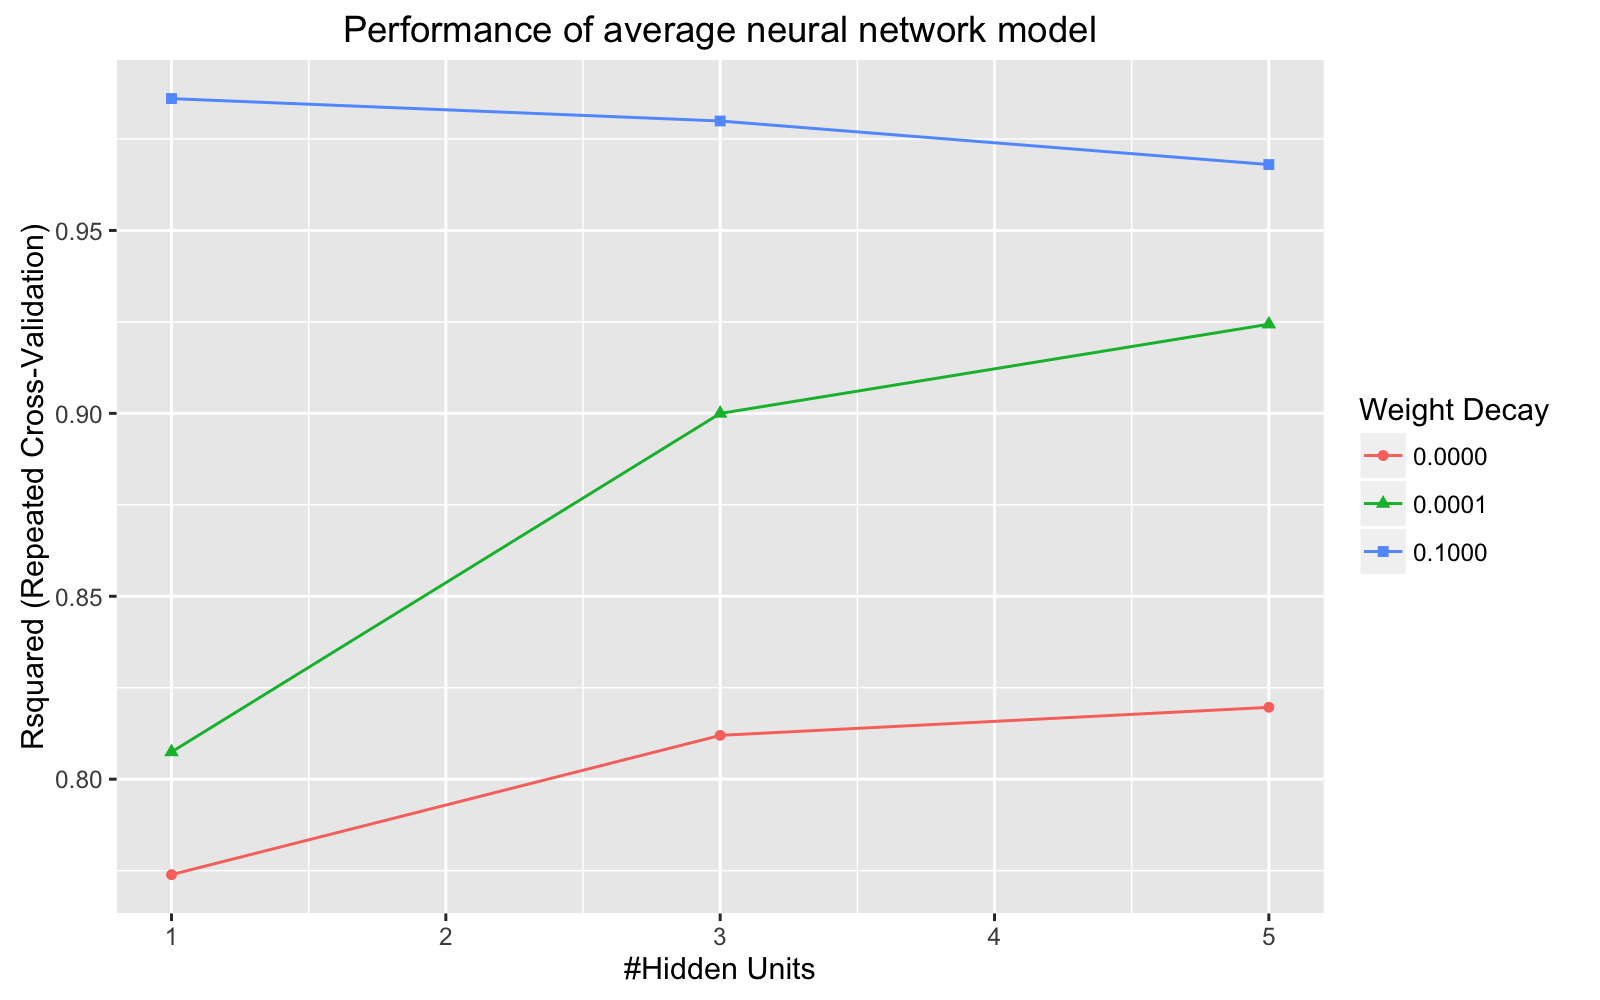
\includegraphics[width=0.5\textwidth]{avgnnet_rsqr.png}
    \caption{Parameter tuning results for Neural network}
    \label{res:ann_tune}
\end{figure}
\begin{figure}[!h]
    \centering
    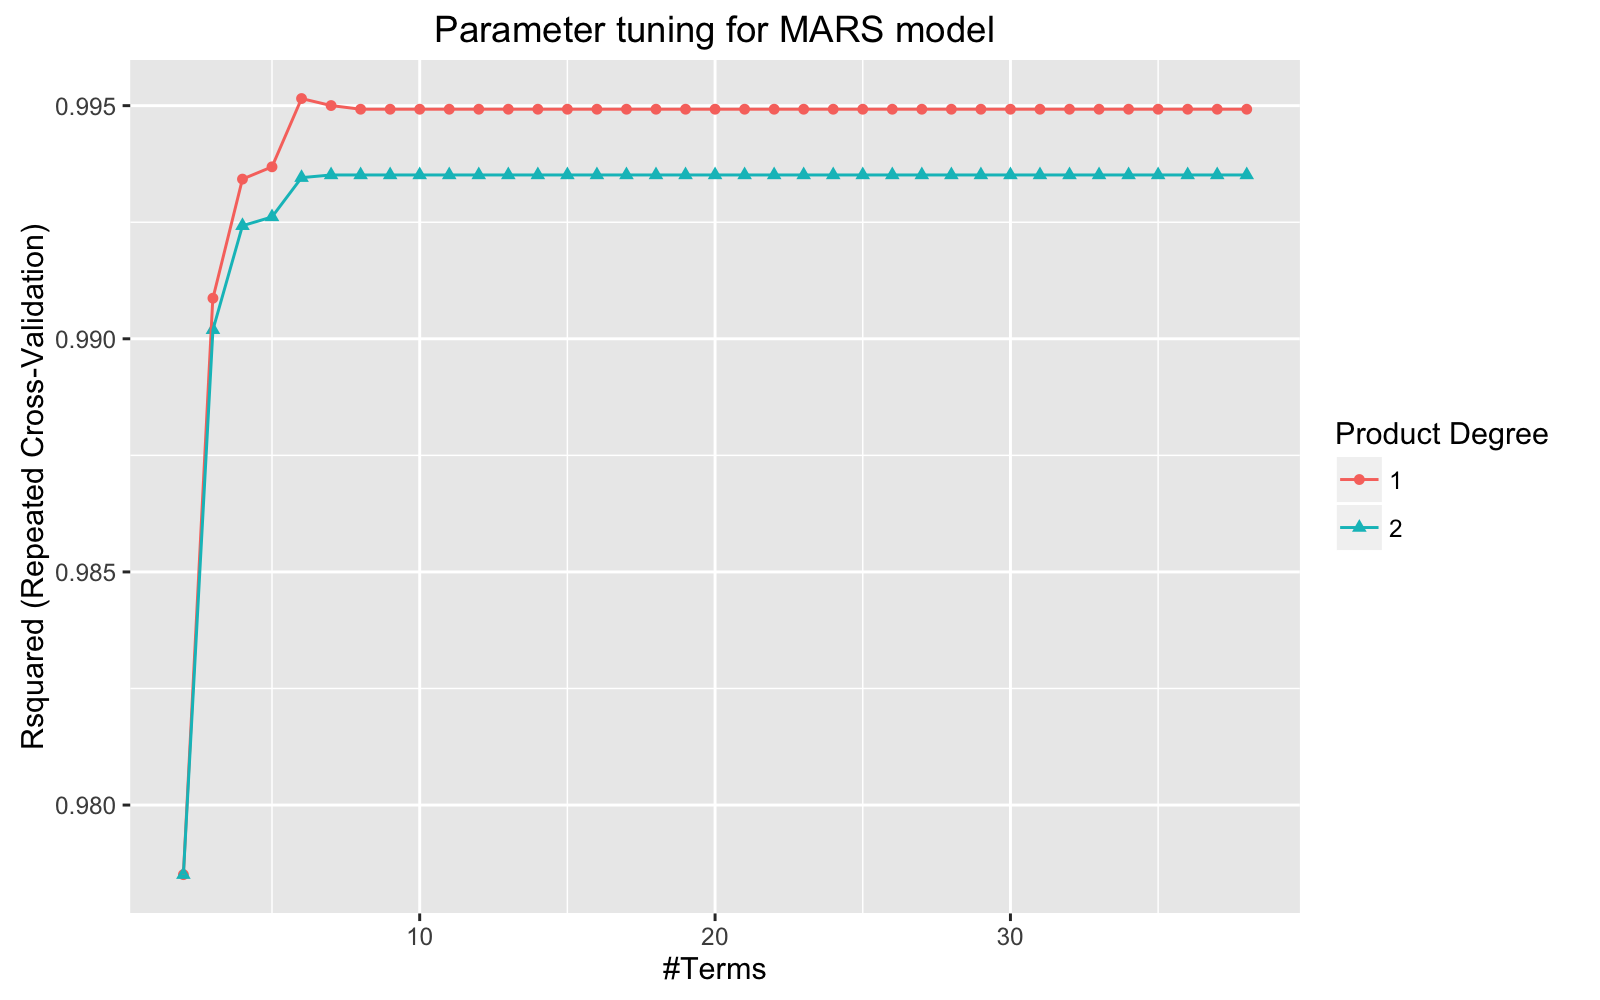
\includegraphics[width=0.5\textwidth]{mars_rsqr.png}
    \caption{Parameter tuning results for MARS}
    \label{res:mars_tune}
\end{figure}

As can be seen in Figures \ref{res:ann_train} and \ref{res:mars_train}, both models fit the training data well with RMSE errors staying pretty low and the coefficient of regression fit, $R^2$, at around 0.98. One might be inclined to argue that such good of a fit might point towards over-fitting, which would very well have been true if not for the k-fold cross validation used during the training process which ensures none of the model parameters have been biased for a specific data point.
\begin{figure}[!h]
    \centering
    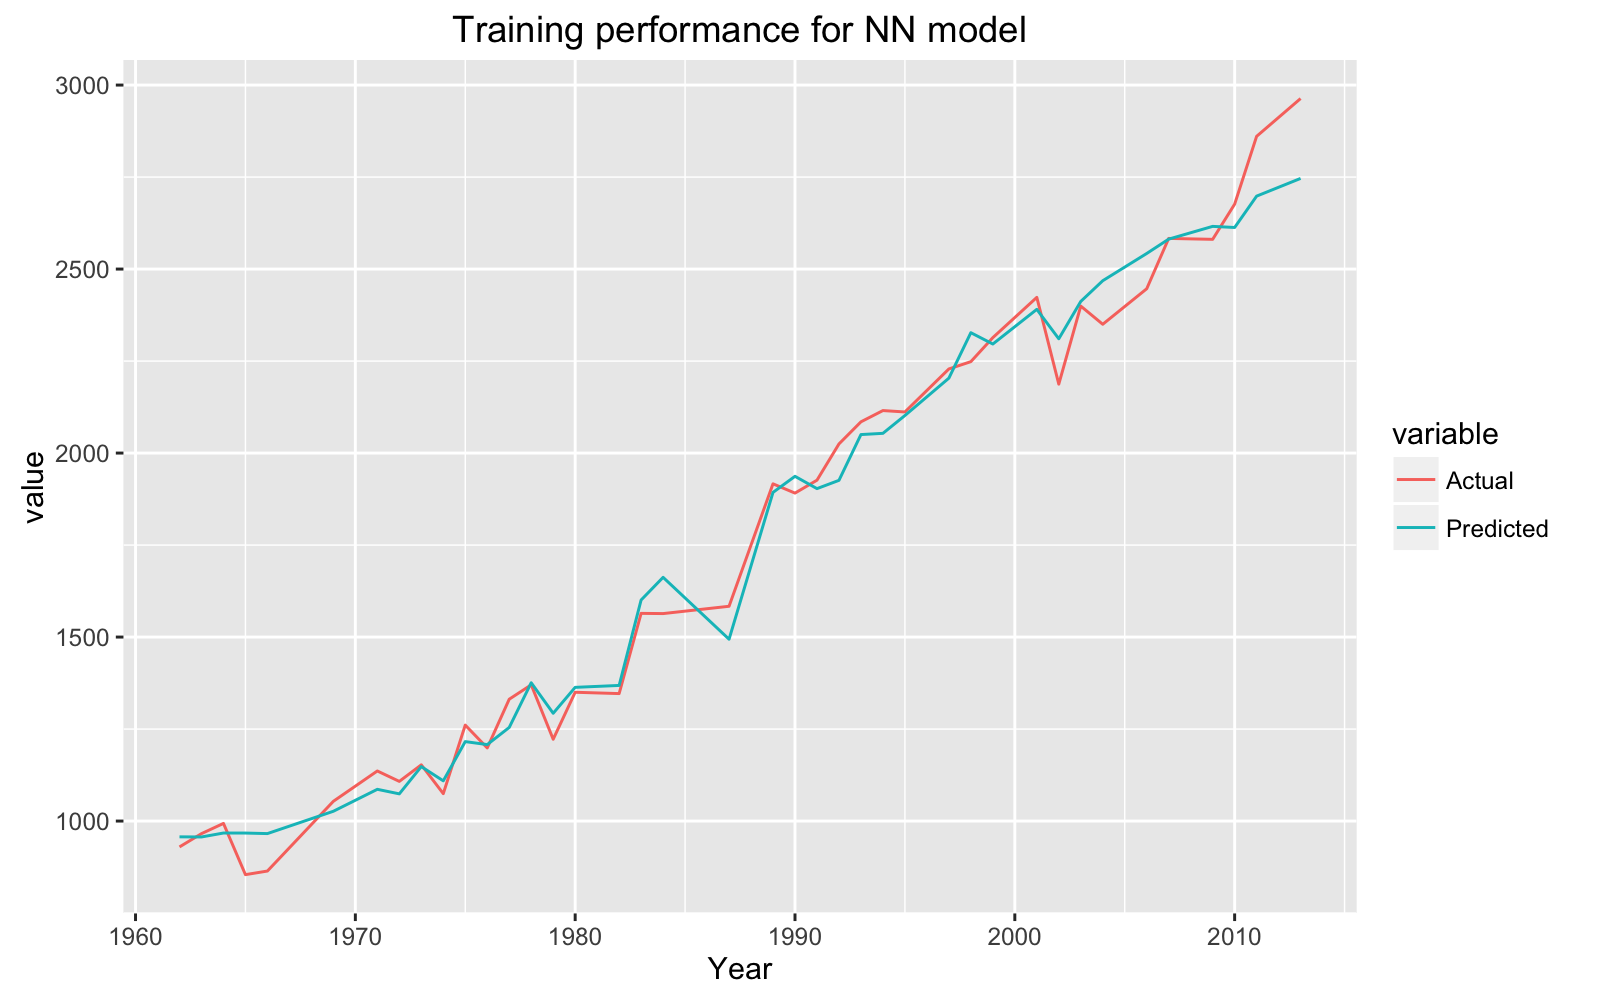
\includegraphics[width=0.5\textwidth]{avgnnet_training.png}
    \caption{Training results for NN}
    \label{res:ann_train}
\end{figure}
\begin{figure}[!h]
    \centering
    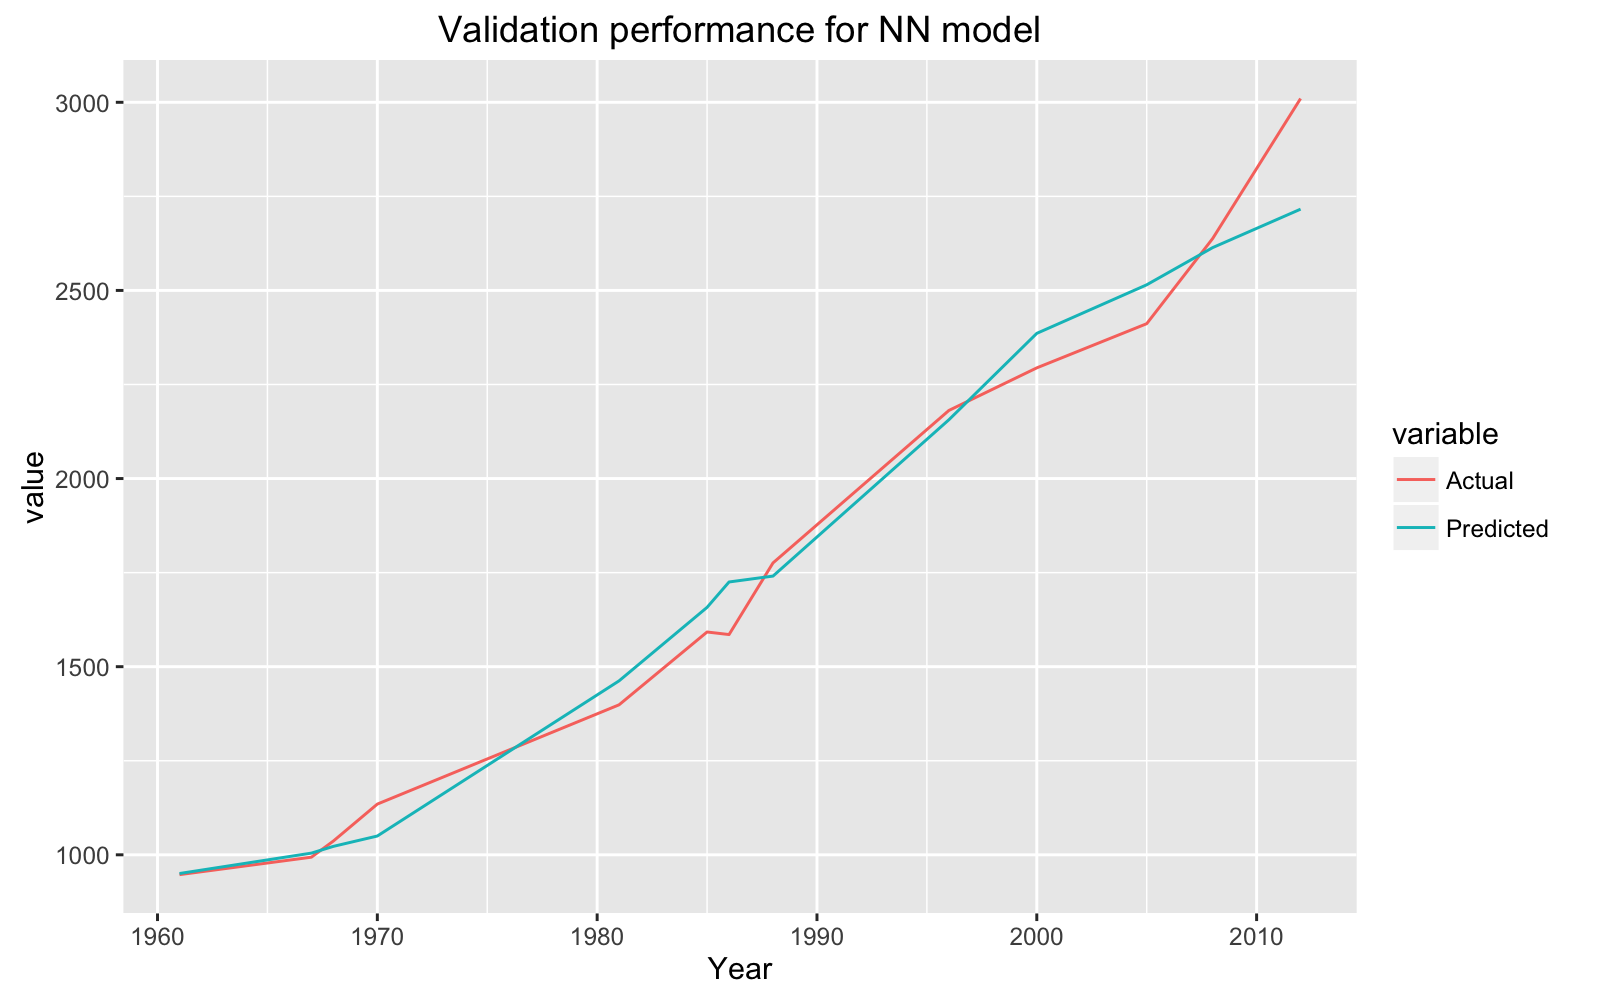
\includegraphics[width=0.5\textwidth]{avgnnet_validate.png}
    \caption{Validation results for NN}
    \label{res:ann_test}
\end{figure}

Figures \ref{res:ann_test} and \ref{res:mars_test} show the prediction accuracy of the models on the validation dataset. Once again, the predictions closely followed the actual values proving the efficacy of these models in predicting crop yield.
\begin{figure}[!h]
    \centering
    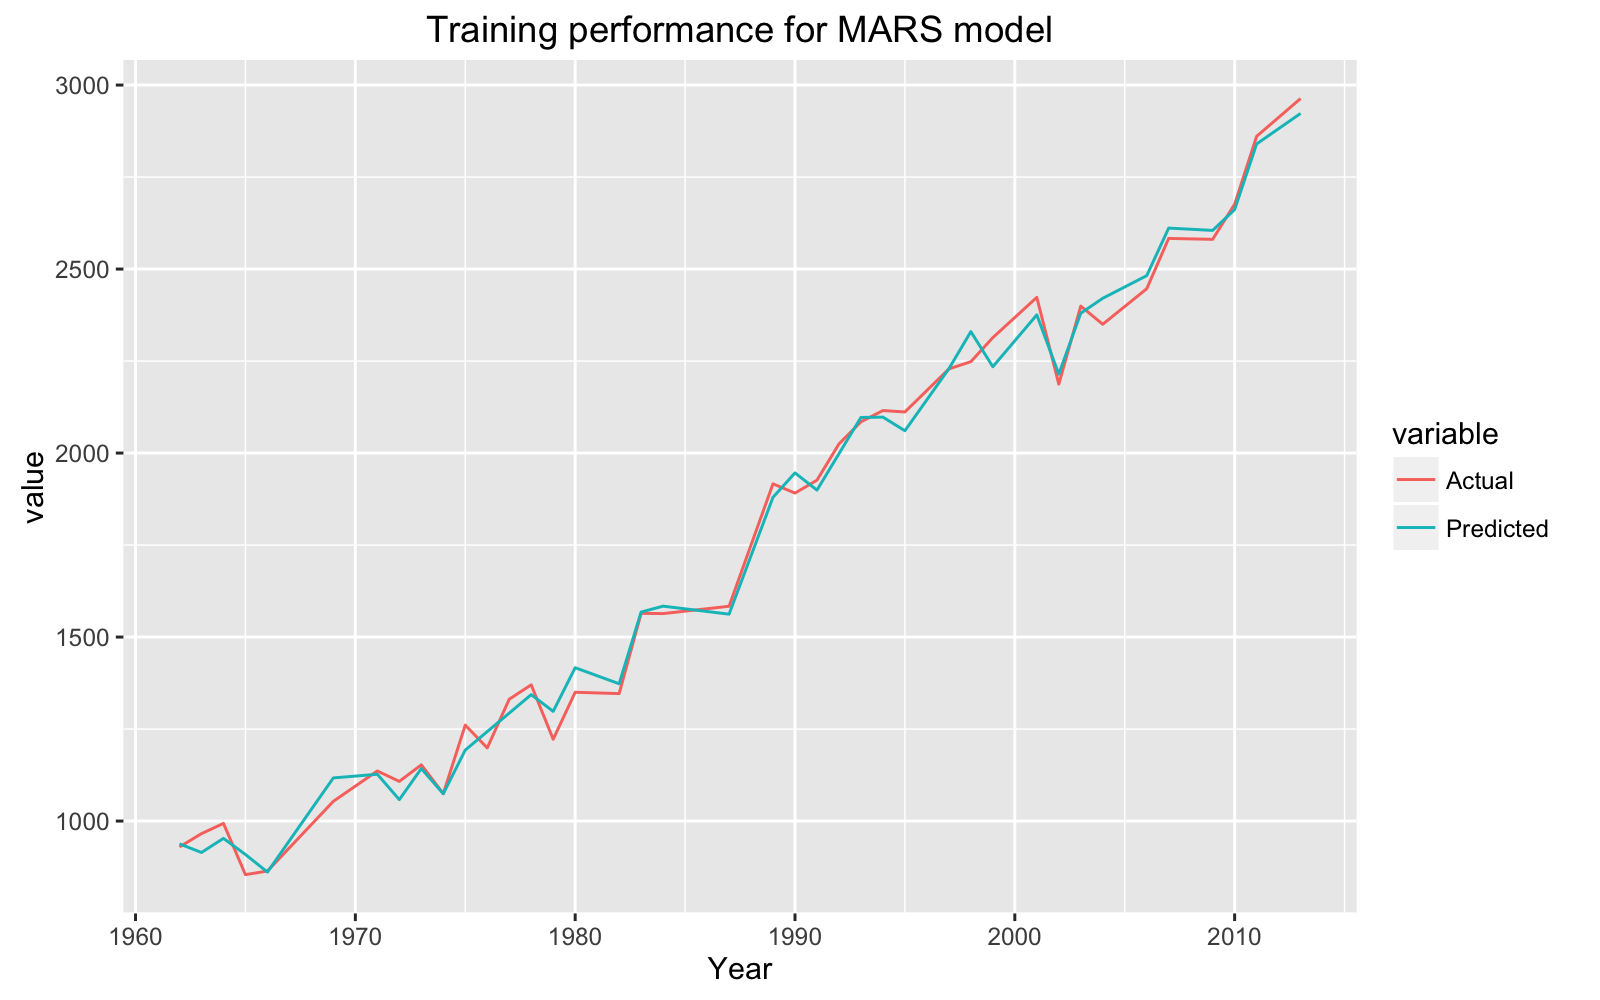
\includegraphics[width=0.5\textwidth]{mars_training.png}
    \caption{Training results for MARS}
    \label{res:mars_train}
\end{figure}
\begin{figure}[!h]
    \centering
    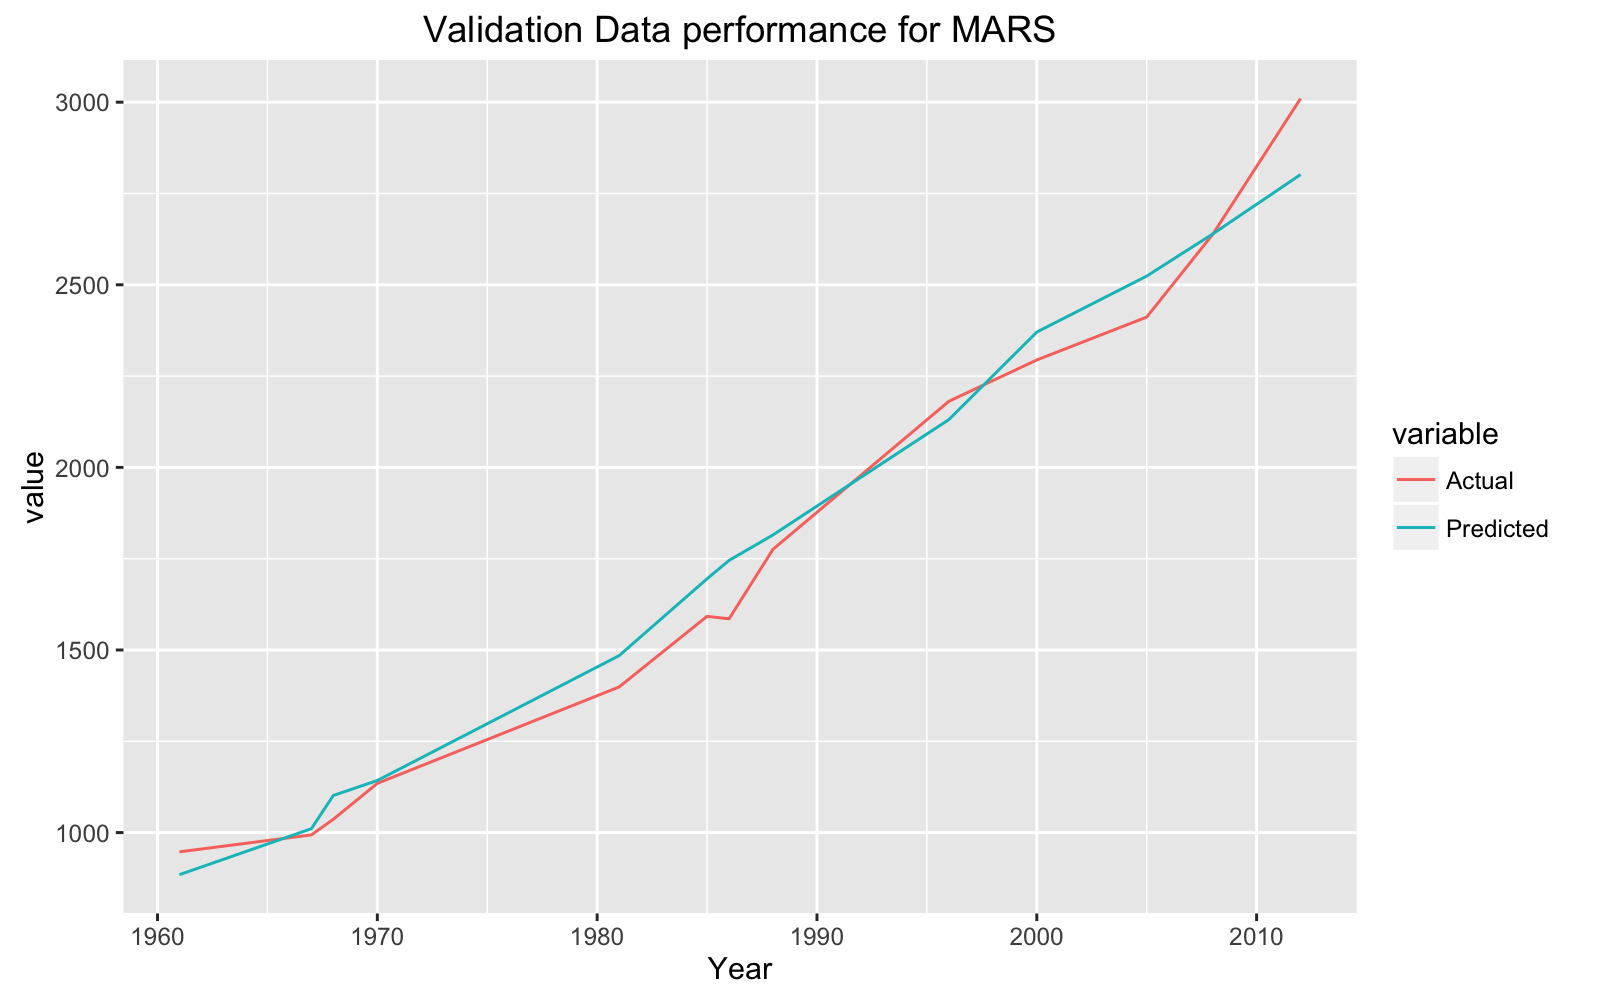
\includegraphics[width=0.5\textwidth]{mars_validate.png}
    \caption{Validation results for MARS}
    \label{res:mars_test}
\end{figure}
% \clearpage
The RMSE and $R^2$ results for the training, Table \ref{tab:res_train}, and testing, Table \ref{tab:res_test}, data-splits for both MARS and Neural Networks have been provided. As is obvious from them, both models had extremely similar performance in fitting the validation data to the model. The low RMSE values, which range from 4-8\% of the mean yield value, indicate really good performance for these models. 
%latex.default(res_training, file = "train_results.tex")%
\begin{table}[!tbp]
\begin{center}
\begin{tabular}{lrr}
\hline\hline
\multicolumn{1}{l}{res}&\multicolumn{1}{c}{rmse}&\multicolumn{1}{c}{r2}\tabularnewline
\hline
AvgNN&$71.8543768205759$&$0.986877633023676$\tabularnewline
MARS&$41.7083829642748$&$0.995445879757786$\tabularnewline
\hline
\end{tabular}\end{center}
\caption{RMSE and $R^2$ results for training}
\label{tab:res_train}
\end{table} 

%latex.default(res_testing, file = "testing_results.tex")%
\begin{table}[!tbp]
\begin{center}
\begin{tabular}{lrr}
\hline\hline
\multicolumn{1}{l}{res}&\multicolumn{1}{c}{rmse}&\multicolumn{1}{c}{r2}\tabularnewline
\hline
AvgNN&$105.0088152187575$&$0.975009493599273$\tabularnewline
MARS&$ 95.1923222679583$&$0.981305690867502$\tabularnewline
\hline
\end{tabular}\end{center}
\caption{RMSE and $R^2$ results for testing}
\label{tab:res_test}
\end{table}

\section{Summary and Conclusions}
\subsection{Software and code}
All the code used to run the analysis and generate the relevant figures, etc., is available on github \cite{Prajna2016}. All the software was written using the statistical programming language R, and all visualizations were generated using the software package \emph{ggplot2}. All the analysis and model training was done using the package \emph{caret \cite{caret2016}}. The files \emph{explore.R} and \emph{analysis.R} document the exploratory and analytical portions of this study. All the figures in this study are completely reproducible using the code provided in the github repository at \url{https://github.com/prajnak/syde522_project}
\subsection{Conclusions}
In conclusion, we found that the models trained here, based on neural networks and Multiple Adaptive Regressive Splines, were able to accurately represent the behavior of the annual crop yields for cereals in India. An assessment of the variables deemed to be important by these models is provided in Figures \ref{res:mars_imp} and \ref{res:avgnn_imp}.
\begin{figure}[!h]
    \centering
    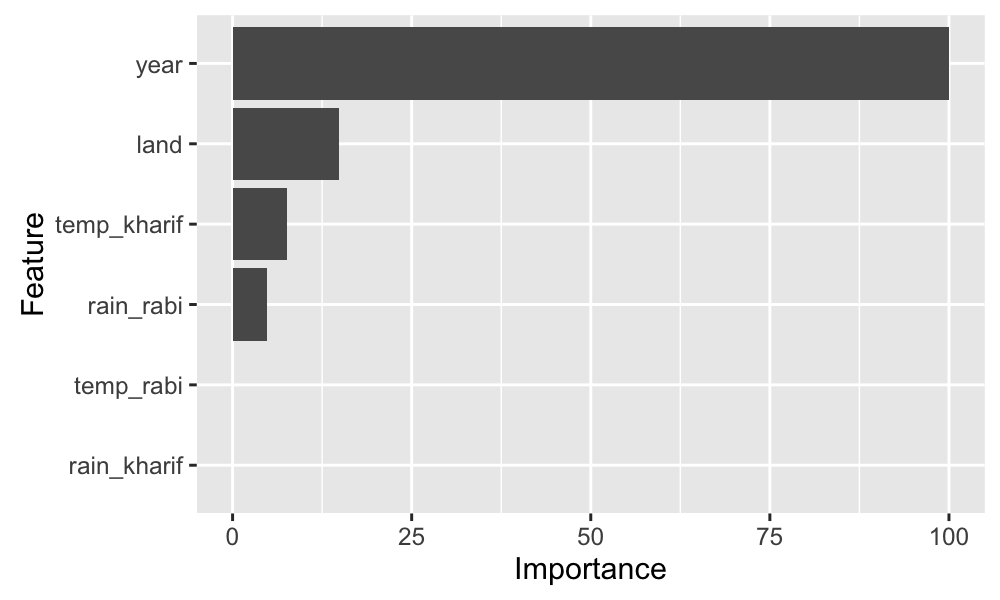
\includegraphics[width=0.5\textwidth]{mars_varimp.png}
    \caption{Important variables in MARS model}
    \label{res:mars_imp}
\end{figure}
\begin{figure}[!h]
    \centering
    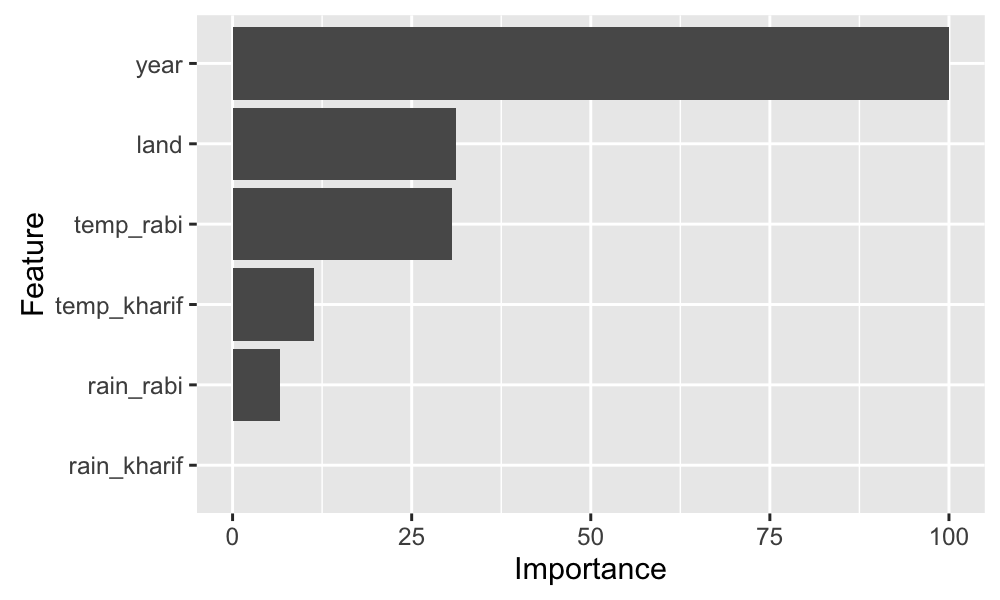
\includegraphics[width=0.5\textwidth]{avgnn_varimp.png}
    \caption{Important variables in NN model}
    \label{res:avgnn_imp}
\end{figure}

These results indicate that the year variable was most important in predicting future crop yields. This makes sense when one can think about the year acting as a proxy for the actual factor driving crop yield higher every year - population. It would be very interesting to run the same analysis using country population instead of the year and verify this claim. Other noticeable aspects include the negligible importance of the rain variables in predicting crop yields. This maybe attributed to large regional variations in precipitation which are lost when one considers aggregated weather data at national scales. It is very likely that the regions responsible for most of the cereal production received much higher rainfall than represented by the seasonal mean values used in this study. 

Previous works have suggested that climatic variables can account for most of the variations in crop yields. Lobell et al.(2010) found that the performance of statistical models differed by climate variable and spatial scale, with time-series statistical models ably reproducing site-specific yield response to precipitation change, but performing less well for temperature responses. The models based on multiple sites were also much less sensitive to the length of historical period used for training. For all three statistical approaches, the performance improved when individual sites were first aggregated to country-level averages. Results suggest that statistical models, as compared to CERES-Maize, represent a useful if imperfect tool for projecting future yield responses, with their usefulness higher at broader spatial scales. It is also at these broader scales that climate projections are most available and reliable, and therefore statistical models are likely to continue to play an important role in anticipating future impacts of climate change \cite{Lobell2010}.

Thus, it is recommended that better national scale predictor aggregates be obtained primarily from the major regions responsible for cereal production in India, including temperature, rainfall and fertilizer intake to obtain much better results as suggested by Lobell et. al. Other recommendations include adding energy usage by the agricultural sector and irrigation levels, using techniques that allow extrapolation of missing data for the variables that were dropped during the data pre-processing stage of this study like agricultural machines and fertilizer uptake. Researchers have found fertilizer uptake, to be an especially useful factor for predicting crop yields as it is also linked to popular crop strains and breeding practices that may vary regionally. Gonzalez-Sanchez et. al found that M5-prime regression trees performed really well, which can be another model to build using this dataset \cite{Gonzalez-Sanchez2014}.

Finally, it is necessary to point out that this work deals only with comparing the predictive accuracy of the above-mentioned techniques. Several factors like model structure, knowledge representation, implementation cost and training time affect the performance of machine learning techniques and further research needs to be done to compare the characteristics of the ML models with agricultural planning factors.

% use section* for acknowledgement
\section*{Acknowledgment}
The author would like to thank H.R. Tizhoosh, Professor, Systems Design Engineering, University of Waterloo for his suggestions about ensuring enough data is available to perform the analysis conducted here but on a regional or smaller spatial scale. The original intent of this report was to use regional climate, soil and fertilizer data and perform analysis at a much smaller spatial scale with the same temporal scale. However, technical difficulties prevented such analyses and the spatial scale had to be increased to the national level to proceed.

\bibliographystyle{IEEEtran}
% \renewcommand{\bibname}{References}
\bibliography{Latex_Template.bib}

% that's all folks
\end{document}


